% CDT503 期末项目报告。编译：在 cdt503/report 下运行 tectonic main.tex（或在 TeXPage 上用 pdfLaTeX）。
% 图片默认从 ../figures/ 读取；上传到 TeXPage 时把 figures 文件夹放在 main.tex 旁边也可以（见 \graphicspath）。
\documentclass[conference]{IEEEtran}
\usepackage[T1]{fontenc}
\usepackage{amsmath,amssymb}
\usepackage{graphicx}
\usepackage{booktabs}
\usepackage{multirow}
\usepackage{xcolor}
\usepackage{tikz}
\usetikzlibrary{positioning,arrows.meta}
\usepackage[hidelinks]{hyperref}
\usepackage{cite}
\graphicspath{{../figures/}{figures/}}

\newcommand{\figwidth}{\columnwidth}

\begin{document}

\title{Beyond Star Ratings:\\Aspect Extraction from Chinese Reviews}

\author{\IEEEauthorblockN{Han Daiyuan (3231363) \qquad Li Mingtai (3231959)}
\IEEEauthorblockA{CDT503 Final Group Project (Track B: NLP / PEFT)\\
Lingnan University, Hong Kong}}

\maketitle

\begin{abstract}
Online shops receive thousands of free-text reviews, but merchants need structured signals: \emph{which} aspect of a
product is praised or criticised. We build a working prototype that turns a Chinese e-commerce review into a JSON
record of its overall sentiment and up to 16 aspect--sentiment pairs. Instead of paying human annotators, a 30B-parameter
teacher (Qwen3-30B-A3B) labels 2{,}425 real reviews under a written annotation guideline; labels that are malformed or
contradict the review's human star rating are filtered out, and a 1.7B student (Qwen3-1.7B) is fine-tuned with LoRA on
an Apple-silicon laptop using MLX. A one-factor-at-a-time sweep over rank, learning rate and adapted layers (10 runs,
selected on validation data only) raises test aspect-F1 from 0.734 to 0.807 ($+0.073$, 95\% bootstrap CI
$[+0.038, +0.110]$; 0.790--0.807 across three training seeds), versus 0.513 for the untuned base model; showing the base model the teacher's four worked
examples instead helps far less (validation F1 0.538 $\rightarrow$ 0.594, vs.\ 0.802 for LoRA). On 100 never-used reviews
labelled by two group members, the student is statistically indistinguishable from the teacher (0.701 vs.\ 0.689
aspect-F1) with 18$\times$ fewer total parameters (under 2$\times$ fewer active ones), about 5$\times$ less weight memory
and 1.8$\times$ the speed. A Gradio demo shows the base and fine-tuned outputs side by side and survived a 12-user
concurrency test.
\end{abstract}

\begin{IEEEkeywords}
aspect-based sentiment analysis, LoRA, knowledge distillation, parameter-efficient fine-tuning, large language models
\end{IEEEkeywords}

% =====================================================================
\section{Introduction and Problem Setup}

Star ratings tell a merchant \emph{whether} customers are happy, but not \emph{why}. A review such as
``\textit{the hotel is close to the metro, but the room has poor sound insulation and check-in took half an hour}''
contains three actionable signals (location $+$, room $-$, service $-$) hidden in one sentence. Extracting such
aspect--sentiment pairs is the classic aspect-based sentiment analysis (ABSA) task~\cite{pontiki2014semeval}.
Our goal is a small model that outputs this information as \emph{machine-readable JSON}, so that a downstream
program can aggregate it (e.g.\ ``40\% of complaints this month are about logistics'').

\textbf{Why not just prompt a large model?} A 30B model follows the format well but is slow and memory-hungry; a 1.7B
model is fast but, when prompted, frequently invents aspect names outside the allowed list or uses a ``neutral'' label the
schema does not permit. Our question is whether parameter-efficient fine-tuning can give the small model the
large model's reliability at the small model's cost.

\textbf{Data.} We use \texttt{online\_shopping\_10\_cats}~\cite{chinesenlpcorpus}, 62{,}774 real Chinese reviews from 10
product categories, each with a binary human sentiment label (Table~\ref{tab:data}). The data are genuinely ``dirty'':
missing texts, byte-order marks, duplicates, copy-pasted promotional templates, and long rants. After removing empty and
duplicate texts and keeping reviews of 12--160 characters, 54{,}472 remain. We draw a stratified sample of 2{,}425
(balanced by category and sentiment) for distillation.

\textbf{Output schema.} Each review maps to
\texttt{\{"overall": pos|neg, "aspects": [\{"aspect", "opinion", "sentiment"\}]\}}, where \emph{aspect} must come from a
fixed list of 16 (e.g.\ Performance, Build \& material, Defect, Logistics, Service, Taste, Room \& facilities) and
\emph{opinion} is a short span copied from the review. A fixed list makes outputs comparable and scoreable.

\begin{table}[t]
\centering
\caption{Dataset statistics.}
\label{tab:data}
\setlength{\tabcolsep}{4pt}
\begin{tabular}{lr}
\toprule
Raw reviews, 10 product categories & 62{,}774 \\
\quad human label positive / negative & 31{,}728 / 31{,}046 \\
After cleaning (unique, 12--160 characters) & 54{,}472 \\
Stratified sample labelled by the teacher & 2{,}425 \\
\quad rejected: invalid JSON / sentiment mismatch & 15 / 182 \\
Kept for training and evaluation & 2{,}228 \\
\quad train / validation / test & 1{,}824 / 142 / 262 \\
Mean review length (characters) & 48.8 \\
Mean aspects per review (teacher labels) & 1.71 \\
Fresh human-labelled reviews (never used) & 100 \\
\bottomrule
\end{tabular}
\end{table}

% =====================================================================
\section{Methodology and Architecture}

Fig.~\ref{fig:pipeline} shows the full system. Every stage runs on one laptop (Apple M5, 32\,GB unified memory).

\begin{figure*}[t]
\centering
\resizebox{\textwidth}{!}{% 系统流程框图（报告图 1）。main.tex 里用 % 系统流程框图（报告图 1）。main.tex 里用 % 系统流程框图（报告图 1）。main.tex 里用 \input{fig_pipeline} 引入，需要 tikz 及 positioning、arrows.meta 库。
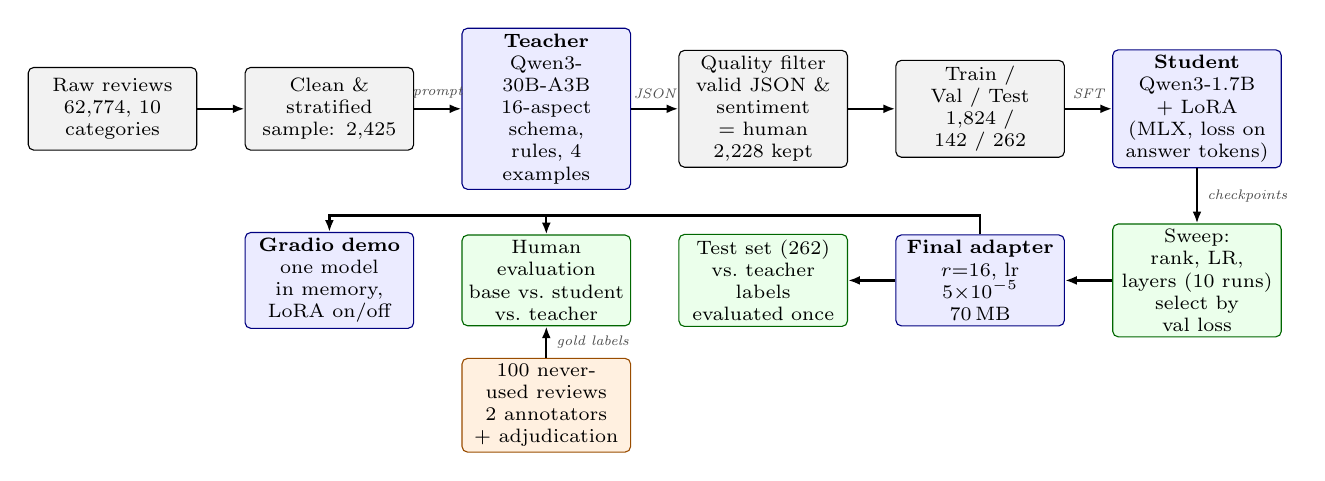
\begin{tikzpicture}[
    node distance=3mm and 6mm,
    box/.style={draw, rounded corners=2pt, align=center, font=\scriptsize, minimum height=10.5mm,
                text width=20mm, inner sep=2pt},
    data/.style={box, fill=gray!10},
    model/.style={box, fill=blue!8, draw=blue!50!black},
    human/.style={box, fill=orange!12, draw=orange!60!black},
    eval/.style={box, fill=green!8, draw=green!40!black},
    arr/.style={-{Latex[length=1.5mm]}, thick},
    lab/.style={font=\tiny\itshape, text=black!70},
  ]
  % ---- 第一排：训练数据和训练（从左到右）----
  \node[data] (raw) {Raw reviews\\62{,}774, 10 categories};
  \node[data, right=of raw] (clean) {Clean \& stratified\\sample: 2{,}425};
  \node[model, right=of clean] (teacher) {\textbf{Teacher}\\Qwen3-30B-A3B\\16-aspect schema,\\rules, 4 examples};
  \node[data, right=of teacher] (filter) {Quality filter\\valid JSON \&\\sentiment = human\\2{,}228 kept};
  \node[data, right=of filter] (split) {Train / Val / Test\\1{,}824 / 142 / 262};
  \node[model, right=of split] (student) {\textbf{Student}\\Qwen3-1.7B + LoRA\\(MLX, loss on\\answer tokens)};
  \draw[arr] (raw) -- (clean);
  \draw[arr] (clean) -- node[lab, above] {prompt} (teacher);
  \draw[arr] (teacher) -- node[lab, above] {JSON} (filter);
  \draw[arr] (filter) -- (split);
  \draw[arr] (split) -- node[lab, above] {SFT} (student);

  % ---- 第二排：选模型，然后三种用途（从右到左）----
  \node[eval, below=7mm of student] (sweep) {Sweep: rank, LR,\\layers (10 runs)\\select by val loss};
  \node[model, left=of sweep] (final) {\textbf{Final adapter}\\$r{=}16$, lr $5{\times}10^{-5}$\\70\,MB};
  \node[eval, left=of final] (test) {Test set (262)\\vs.\ teacher labels\\evaluated once};
  \node[eval, left=of test] (heval) {Human evaluation\\base vs.\ student\\vs.\ teacher};
  \node[model, left=of heval] (demo) {\textbf{Gradio demo}\\one model in memory,\\LoRA on/off};
  \draw[arr] (student) -- node[lab, right] {checkpoints} (sweep);
  \draw[arr] (sweep) -- (final);
  \draw[arr] (final) -- (test);
  % 最终模型到人工评估、演示的箭头从两排之间绕过去
  \draw[arr] (final.north) -- ++(0,2.4mm) -| (heval.north);
  \draw[arr] (final.north) -- ++(0,2.4mm) -| (demo.north);

  % ---- 第三排：人工标注，评论来自从没用过的那部分数据 ----
  \node[human, below=4mm of heval] (fresh) {100 never-used reviews\\2 annotators\\+ adjudication};
  \draw[arr] (fresh) -- node[lab, right] {gold labels} (heval);
\end{tikzpicture}
 引入，需要 tikz 及 positioning、arrows.meta 库。
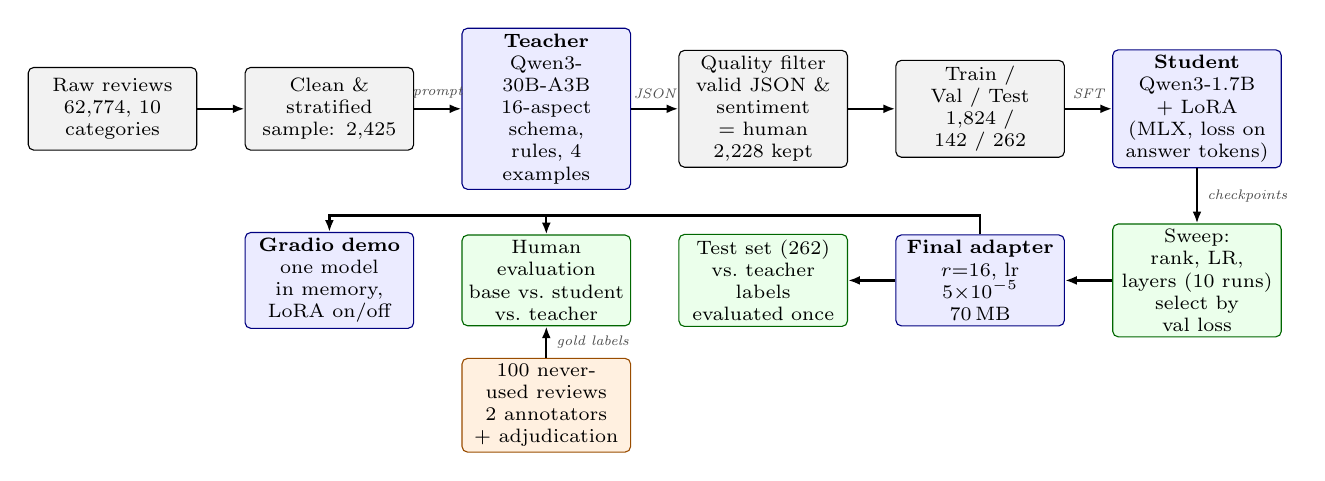
\begin{tikzpicture}[
    node distance=3mm and 6mm,
    box/.style={draw, rounded corners=2pt, align=center, font=\scriptsize, minimum height=10.5mm,
                text width=20mm, inner sep=2pt},
    data/.style={box, fill=gray!10},
    model/.style={box, fill=blue!8, draw=blue!50!black},
    human/.style={box, fill=orange!12, draw=orange!60!black},
    eval/.style={box, fill=green!8, draw=green!40!black},
    arr/.style={-{Latex[length=1.5mm]}, thick},
    lab/.style={font=\tiny\itshape, text=black!70},
  ]
  % ---- 第一排：训练数据和训练（从左到右）----
  \node[data] (raw) {Raw reviews\\62{,}774, 10 categories};
  \node[data, right=of raw] (clean) {Clean \& stratified\\sample: 2{,}425};
  \node[model, right=of clean] (teacher) {\textbf{Teacher}\\Qwen3-30B-A3B\\16-aspect schema,\\rules, 4 examples};
  \node[data, right=of teacher] (filter) {Quality filter\\valid JSON \&\\sentiment = human\\2{,}228 kept};
  \node[data, right=of filter] (split) {Train / Val / Test\\1{,}824 / 142 / 262};
  \node[model, right=of split] (student) {\textbf{Student}\\Qwen3-1.7B + LoRA\\(MLX, loss on\\answer tokens)};
  \draw[arr] (raw) -- (clean);
  \draw[arr] (clean) -- node[lab, above] {prompt} (teacher);
  \draw[arr] (teacher) -- node[lab, above] {JSON} (filter);
  \draw[arr] (filter) -- (split);
  \draw[arr] (split) -- node[lab, above] {SFT} (student);

  % ---- 第二排：选模型，然后三种用途（从右到左）----
  \node[eval, below=7mm of student] (sweep) {Sweep: rank, LR,\\layers (10 runs)\\select by val loss};
  \node[model, left=of sweep] (final) {\textbf{Final adapter}\\$r{=}16$, lr $5{\times}10^{-5}$\\70\,MB};
  \node[eval, left=of final] (test) {Test set (262)\\vs.\ teacher labels\\evaluated once};
  \node[eval, left=of test] (heval) {Human evaluation\\base vs.\ student\\vs.\ teacher};
  \node[model, left=of heval] (demo) {\textbf{Gradio demo}\\one model in memory,\\LoRA on/off};
  \draw[arr] (student) -- node[lab, right] {checkpoints} (sweep);
  \draw[arr] (sweep) -- (final);
  \draw[arr] (final) -- (test);
  % 最终模型到人工评估、演示的箭头从两排之间绕过去
  \draw[arr] (final.north) -- ++(0,2.4mm) -| (heval.north);
  \draw[arr] (final.north) -- ++(0,2.4mm) -| (demo.north);

  % ---- 第三排：人工标注，评论来自从没用过的那部分数据 ----
  \node[human, below=4mm of heval] (fresh) {100 never-used reviews\\2 annotators\\+ adjudication};
  \draw[arr] (fresh) -- node[lab, right] {gold labels} (heval);
\end{tikzpicture}
 引入，需要 tikz 及 positioning、arrows.meta 库。
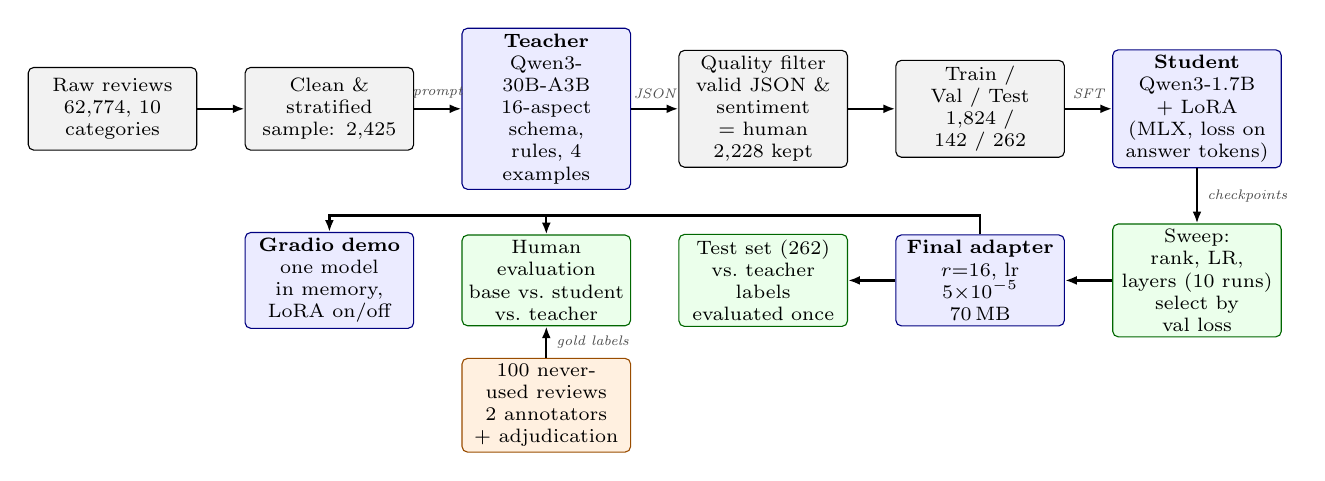
\begin{tikzpicture}[
    node distance=3mm and 6mm,
    box/.style={draw, rounded corners=2pt, align=center, font=\scriptsize, minimum height=10.5mm,
                text width=20mm, inner sep=2pt},
    data/.style={box, fill=gray!10},
    model/.style={box, fill=blue!8, draw=blue!50!black},
    human/.style={box, fill=orange!12, draw=orange!60!black},
    eval/.style={box, fill=green!8, draw=green!40!black},
    arr/.style={-{Latex[length=1.5mm]}, thick},
    lab/.style={font=\tiny\itshape, text=black!70},
  ]
  % ---- 第一排：训练数据和训练（从左到右）----
  \node[data] (raw) {Raw reviews\\62{,}774, 10 categories};
  \node[data, right=of raw] (clean) {Clean \& stratified\\sample: 2{,}425};
  \node[model, right=of clean] (teacher) {\textbf{Teacher}\\Qwen3-30B-A3B\\16-aspect schema,\\rules, 4 examples};
  \node[data, right=of teacher] (filter) {Quality filter\\valid JSON \&\\sentiment = human\\2{,}228 kept};
  \node[data, right=of filter] (split) {Train / Val / Test\\1{,}824 / 142 / 262};
  \node[model, right=of split] (student) {\textbf{Student}\\Qwen3-1.7B + LoRA\\(MLX, loss on\\answer tokens)};
  \draw[arr] (raw) -- (clean);
  \draw[arr] (clean) -- node[lab, above] {prompt} (teacher);
  \draw[arr] (teacher) -- node[lab, above] {JSON} (filter);
  \draw[arr] (filter) -- (split);
  \draw[arr] (split) -- node[lab, above] {SFT} (student);

  % ---- 第二排：选模型，然后三种用途（从右到左）----
  \node[eval, below=7mm of student] (sweep) {Sweep: rank, LR,\\layers (10 runs)\\select by val loss};
  \node[model, left=of sweep] (final) {\textbf{Final adapter}\\$r{=}16$, lr $5{\times}10^{-5}$\\70\,MB};
  \node[eval, left=of final] (test) {Test set (262)\\vs.\ teacher labels\\evaluated once};
  \node[eval, left=of test] (heval) {Human evaluation\\base vs.\ student\\vs.\ teacher};
  \node[model, left=of heval] (demo) {\textbf{Gradio demo}\\one model in memory,\\LoRA on/off};
  \draw[arr] (student) -- node[lab, right] {checkpoints} (sweep);
  \draw[arr] (sweep) -- (final);
  \draw[arr] (final) -- (test);
  % 最终模型到人工评估、演示的箭头从两排之间绕过去
  \draw[arr] (final.north) -- ++(0,2.4mm) -| (heval.north);
  \draw[arr] (final.north) -- ++(0,2.4mm) -| (demo.north);

  % ---- 第三排：人工标注，评论来自从没用过的那部分数据 ----
  \node[human, below=4mm of heval] (fresh) {100 never-used reviews\\2 annotators\\+ adjudication};
  \draw[arr] (fresh) -- node[lab, right] {gold labels} (heval);
\end{tikzpicture}
}
\caption{System architecture. Top: the teacher labels a stratified sample under a written guideline, a quality filter
removes unreliable labels, and the student is fine-tuned with LoRA. Bottom: a hyper-parameter sweep selects the final
adapter on validation loss; the adapter is then evaluated once on the test set, against fresh human labels, and served in
a Gradio demo that keeps a single model in memory and switches the adapter on and off.}
\label{fig:pipeline}
\end{figure*}

\subsection{Knowledge distillation with a quality filter}
Following the idea of transferring a large model's behaviour into a small one~\cite{hinton2015distilling,hsieh2023distilling}
and the finding that LLMs can be cost-effective annotators~\cite{gilardi2023chatgpt}, we use
Qwen3-30B-A3B~\cite{qwen3} (4-bit, mixture-of-experts: 30.5B parameters, 3.3B active per token) as the teacher. Its prompt contains the
16 aspect definitions, nine disambiguation rules (e.g.\ ``lag or short battery life $\rightarrow$ Performance;
crashes or dead on arrival $\rightarrow$ Defect'') and four worked examples. Labelling the 2{,}425 reviews took
$\approx$50\,min.

Teacher labels are not ground truth, so we keep a label only if (i) it parses as valid JSON with allowed values, and
(ii) its overall sentiment agrees with the dataset's \emph{human} sentiment label. Rule (ii) removed 182 reviews; many
were genuinely mixed (``good water heater, but the installation fee is outrageous'') or mislabelled in the original data.

\subsection{Iterating on the label schema}
Our first schema (12 aspects) produced systematic confusion: a single ``Quality'' aspect mixed build quality, defects
and authenticity, and the teacher kept inventing natural names such as ``texture'' or ``location''. We revised it to 16
aspects whose names are the words people actually use, plus the disambiguation rules above. To check that the new
schema is genuinely clearer---not just different---we had a \emph{second} model (Qwen3-14B) label the same 285 reviews
independently and measured inter-annotator agreement with the teacher: aspect-F1 rose from 0.768 to 0.806 even though
the number of categories grew from 12 to 16, and teacher format errors fell from 40 to 15 per 2{,}425.

\subsection{LoRA fine-tuning}
LoRA~\cite{hu2022lora} freezes each pretrained weight matrix $W_0\in\mathbb{R}^{d\times k}$ and learns a low-rank update:
\begin{equation}
h = W_0 x + s\,B A x,
\label{eq:lora}
\end{equation}
with $B\in\mathbb{R}^{d\times r}$, $A\in\mathbb{R}^{r\times k}$ and rank $r\ll\min(d,k)$. $B$ is initialised to zero so training starts from the base model. In the original formulation $s=\alpha/r$; in
MLX-LM~\cite{mlx2023,mlxlm} the scale $s$ is set directly (default 20). With $r=16$ on the attention and MLP projections
of all 28 layers, only 17.4M of 1{,}720M parameters (1.01\%) are trained and the adapter is 70\,MB.

The prompt (instructions, aspect list and rules, $\approx$780 tokens) is identical for every example, so we compute the
cross-entropy loss only on the answer tokens $y$ (``mask prompt''):
\begin{equation}
\mathcal{L} = -\frac{1}{|y|}\sum_{t=1}^{|y|}\log p_\theta\!\left(y_t \mid \text{prompt}, y_{<t}\right).
\end{equation}

\subsection{Evaluation metrics}
\textbf{JSON validity} is the share of outputs that parse and use only allowed values---a deployed system cannot use
anything else. \textbf{Sentiment accuracy} compares the overall sentiment with the dataset's \emph{human} label.
\textbf{Aspect-F1} is the micro-averaged F1 over (aspect, sentiment) pairs, $F_1 = 2TP/(2TP+FP+FN)$, summed over all
reviews; the opinion span is not scored because wording varies. On the test split the reference is the (filtered)
teacher label; on the fresh set it is the adjudicated human label. Uncertainty is reported as 95\% intervals from 2{,}000
bootstrap resamples of reviews~\cite{efron1993bootstrap}; differences between two models use paired resampling.

\textbf{Data discipline.} Hyper-parameters and checkpoints were chosen on the 142-review validation split only; each
model was scored on the 262-review test split exactly once, after the final configuration was fixed.

% =====================================================================
\section{Implementation and Results}

\subsection{Setup}
Table~\ref{tab:hparams} lists the default configuration. Training 480 steps (2.1 epochs) takes $\approx$94\,min on the
laptop; validation loss is computed every 40 steps and a checkpoint is saved at the same interval.

\begin{table}[t]
\centering
\caption{Default training configuration (MLX-LM 0.32).}
\label{tab:hparams}
\setlength{\tabcolsep}{4pt}
\begin{tabular}{ll}
\toprule
Student & Qwen3-1.7B (bf16), thinking mode off \\
LoRA & $r=16$, $s=20$, dropout 0.05, all 28 layers \\
Optimiser & AdamW, constant LR $10^{-4}$ (tuned: $5{\times}10^{-5}$) \\
Batch / steps & 8 / 480, gradient checkpointing \\
Max sequence & 1{,}280 tokens; loss on answer tokens only \\
Selection & lowest validation loss (checkpoint every 40 steps) \\
\bottomrule
\end{tabular}
\end{table}

\subsection{Main result}
Table~\ref{tab:main} compares the untuned base model, LoRA with the default configuration, and LoRA with the tuned
learning rate. Fine-tuning fixes the format problem (90.8\%$\rightarrow$99.6--100\% valid JSON) and raises
aspect-F1 by 0.220 (CI $[+0.164, +0.277]$); for the selected run (seed 42), tuning adds a further 0.073
(CI $[+0.038, +0.110]$). Inference cost is unchanged at $\approx$0.6\,s per review (batched). These intervals capture
only \emph{which test reviews were sampled}, not training randomness, so we retrained the tuned configuration with two
more seeds (43, 44), again choosing each checkpoint by validation loss. Their test aspect-F1 is 0.790 and 0.805: the
selected run sits at the top of the range, the three-seed mean is 0.801 (Table~\ref{tab:main}), and every seed beats
the default by at least 0.056. The default itself was trained once on these data (a second seed, scored on validation
only, moved F1 by 0.011), so the gain still carries some seed uncertainty on that side.

\textbf{Few-shot prompting and cost.} Table~\ref{tab:cost} compares the alternatives on the validation split under
identical conditions. Showing the base model the teacher's four worked examples raises aspect-F1 only from 0.538 to 0.594
and leaves its 8.5\% invalid outputs unchanged; LoRA reaches 0.802 with no invalid output. The teacher has 17.5$\times$
more parameters than the student, but as a mixture-of-experts model it activates only 3.3B per token, 1.9$\times$ the
student's 1.74B. Its weights take 17.2\,GB versus 3.5\,GB (4.9$\times$; peak memory during generation 19.8 vs.\
5.7\,GB, 3.5$\times$), and it is 1.8$\times$ slower per review.

\begin{table}[t]
\centering
\caption{Test-set results (262 reviews, reference = filtered teacher labels). Each trained model evaluated once.
$^\dagger$Mean of three training seeds, with min--max in parentheses; the selected seed-42 run scores 0.807
(CI 0.773--0.838).}
\label{tab:main}
\setlength{\tabcolsep}{1.8pt}
\begin{tabular}{lccc}
\toprule
Model & JSON valid & Sent.\ acc. & Aspect-F1 (95\% CI) \\
\midrule
Base Qwen3-1.7B & 0.908 & 0.882 & 0.513 (0.463--0.561) \\
LoRA, default ($\text{lr}=10^{-4}$) & \textbf{1.000} & 0.947 & 0.734 (0.698--0.769) \\
LoRA, tuned ($\text{lr}=5{\times}10^{-5}$)$^\dagger$ & 0.997 & \textbf{0.969} & \textbf{0.801} (0.790--0.807) \\
\bottomrule
\end{tabular}
\end{table}

\begin{table}[t]
\centering
\caption{Few-shot baseline and inference cost on the validation split (142 reviews, batch size 8, Apple M5).
$^*$Scored against the teacher's own labels, so not comparable. Batched decoding differs slightly across batch
sizes, hence LoRA's 0.802 here vs.\ 0.793 in Table~\ref{tab:sweep} (batch 16).}
\label{tab:cost}
\setlength{\tabcolsep}{2.5pt}
\begin{tabular}{lccccc}
\toprule
Setting & Params, B & Mem., GB & s/rev. & JSON & Asp.\ F1 \\
 & tot./act. & wts/peak & & & \\
\midrule
Teacher, 4-shot & 30.5/3.3 & 17.2/19.8 & 1.37 & 1.000 & 0.984$^*$ \\
Base 1.7B, 0-shot & 1.72/1.72 & 3.4/5.4 & 0.72 & 0.915 & 0.538 \\
Base 1.7B, 4-shot & 1.72/1.72 & 3.4/5.8 & 0.75 & 0.915 & 0.594 \\
LoRA student & 1.74/1.74 & 3.5/5.7 & 0.75 & \textbf{1.000} & \textbf{0.802} \\
\bottomrule
\end{tabular}
\end{table}

\subsection{Systematic hyper-parameter study}
\label{sec:sweep}
We varied one factor at a time around the default: rank $r\in\{4,8,16,32\}$, learning rate
$\in\{5{\times}10^{-5},10^{-4},2{\times}10^{-4}\}$ and the number of adapted (top) layers $\in\{8,16,28\}$, plus two
diagnostic runs: the default with a different random seed, and $r=32$ with $s=10$ (Table~\ref{tab:sweep},
Fig.~\ref{fig:sweep}). The seed run tells us how much a score moves by chance alone: validation aspect-F1 0.747 vs.\
0.758. Three seeds of the selected configuration, run after the sweep, span 0.788--0.807, so we treat differences
below $\approx$0.02 as noise. Because the validation split has only 142 reviews,
even somewhat larger differences may partly reflect which reviews it happens to contain, so we draw conclusions only
from large effects.

\begin{table}[t]
\centering
\caption{Sweep results on the validation split (142 reviews). Bold: selected configuration.
$^\dagger$Run after selection, to measure seed variation; not used for choosing.}
\label{tab:sweep}
\setlength{\tabcolsep}{2.5pt}
\begin{tabular}{lrrrrr}
\toprule
Run & Params & Best step & Val loss & Asp.\ F1 & Min \\
\midrule
Default ($r{=}16$, lr $10^{-4}$) & 17.4M & 400 & 0.130 & 0.758 & 94 \\
\quad same, seed 43 & 17.4M & 280 & 0.138 & 0.747 & 93 \\
$r=4$ & 4.4M & 440 & 0.118 & 0.780 & 98 \\
$r=8$ & 8.7M & 200 & 0.131 & 0.762 & 96 \\
$r=32$ & 34.9M & 400 & 0.179 & 0.697 & 93 \\
$r=32$, $s=10$ & 34.9M & 400 & 0.135 & 0.766 & 93 \\
\textbf{lr $5{\times}10^{-5}$} & 17.4M & 240 & \textbf{0.115} & \textbf{0.793} & 94 \\
\quad same, seed 43$^\dagger$ & 17.4M & 160 & 0.112 & 0.788 & 96 \\
\quad same, seed 44$^\dagger$ & 17.4M & 280 & 0.115 & 0.807 & 96 \\
lr $2{\times}10^{-4}$ & 17.4M & -- & diverged & 0.000 & 93 \\
Top 8 layers & 5.0M & 320 & 0.144 & 0.749 & 46 \\
Top 16 layers & 10.0M & 200 & 0.126 & 0.760 & 65 \\
\bottomrule
\end{tabular}
\end{table}

\begin{figure*}[t]
\centering
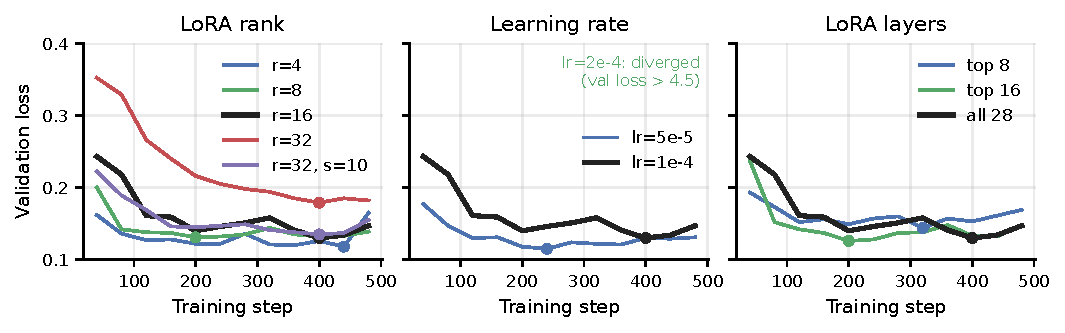
\includegraphics[width=\textwidth]{sweep_val_curves}\\[1mm]
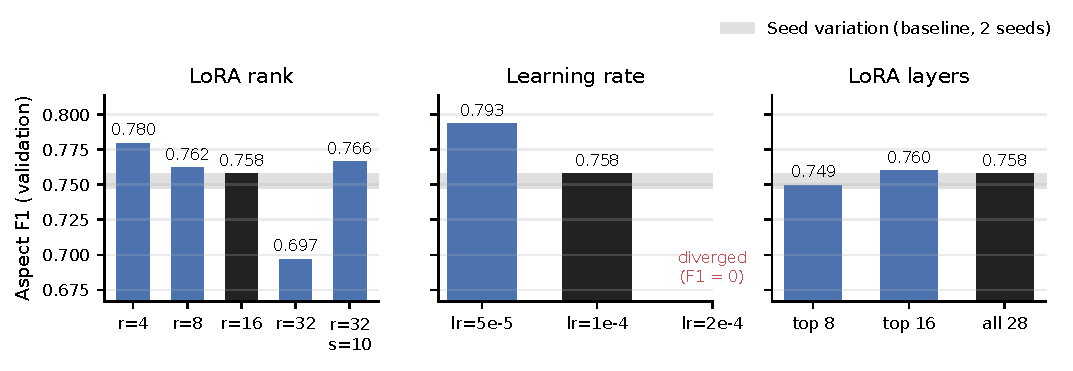
\includegraphics[width=\textwidth]{sweep_metrics}
\caption{One-factor-at-a-time sweep. Top: validation loss during training (dots mark the selected checkpoint).
Bottom: validation aspect-F1 of the selected checkpoint; the grey band is the spread between two seeds of the default
configuration, i.e.\ what chance alone can explain.}
\label{fig:sweep}
\end{figure*}

\textbf{Learning rate matters most.} Halving it to $5\times10^{-5}$ gives the lowest validation loss (0.115) and the
best F1 (0.793, $+0.035$); all three of its seeds (0.788--0.807) beat both seeds of the default (0.747--0.758).
Doubling the learning rate to $2\times10^{-4}$---with a constant
schedule and no warm-up---diverges within 40 steps
(validation loss jumps from 2.6 to 7.1 and the model emits repeated punctuation), never recovering.

\textbf{Larger rank is not better---because of the scale.} $r=32$ is clearly worse (0.697). Since MLX-LM multiplies the
update by a fixed $s$ rather than $\alpha/r$, doubling $r$ also enlarges the effective update. Re-running $r=32$ with
$s=10$, i.e.\ keeping $\alpha=s\,r=320$ constant as in the original LoRA, restores F1 to 0.766, within noise of the
default. This confirms the diagnosis and agrees with work on rank-dependent scaling~\cite{kalajdzievski2023rslora}.
Small ranks are sufficient for this narrow task: $r=4$ (4.4M parameters) scores 0.780.

\textbf{Fewer layers are a free speed-up.} Adapting only the top 8 or 16 layers stays within the noise band while cutting
training time from 94 to 46 or 65 minutes, since back-propagation stops at the lowest adapted layer.

\textbf{Checkpoint selection matters.} Fig.~\ref{fig:loss} shows that at the start of the second epoch the training loss
halves while validation loss stays flat---the model begins to memorise. In none of the eleven converged runs was the final
checkpoint the best one; for $r=4$, validation loss rises from 0.118 at step 440 to 0.165 at step 480.

\begin{figure}[t]
\centering
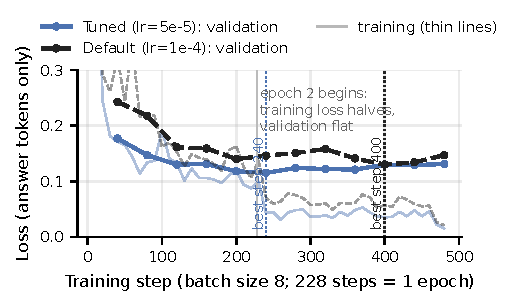
\includegraphics[width=\figwidth]{final_loss_curve}
\caption{Training (thin) and validation (thick) loss for the tuned and default configurations. Dotted lines mark the
checkpoints selected by validation loss.}
\label{fig:loss}
\end{figure}

\subsection{Human evaluation on unseen reviews}
The test split has two weaknesses: its reference labels come from the teacher, and it only contains reviews where the
teacher agreed with the human sentiment label (an ``easier'' subset). We therefore drew 100 reviews that had never been
used anywhere (10 per category, balanced by sentiment) and two group members labelled them with a purpose-built web tool
that hides all model outputs. Twenty reviews were labelled by both annotators; the other 80 by one annotator only.
Agreement on the shared 20 was modest (aspect-F1 0.644), so the two annotators jointly adjudicated the 20 disagreeing or
contradictory items; afterwards each annotator's original labels reached 0.907 and 0.943 F1 against the final labels.

Table~\ref{tab:human} shows that the student clearly beats its base model ($+0.24$, CI $[+0.18, +0.31]$) and is
statistically indistinguishable from the teacher (difference CI $[-0.05, +0.07]$). Sentiment accuracy is lower than on
the test split (0.90 vs.\ 0.97), which confirms that the filtered test set is easier than real-world data.

To compare models with human agreement like for like, Table~\ref{tab:fair} scores every system against each annotator's
\emph{original} labels on the 20 shared reviews. Annotator B agrees with A at 0.644; the student reaches 0.661 on
average, the teacher 0.693 and the base model 0.419. With only 20 reviews the intervals are wide and overlap, so we
cannot tell whether the models are above, at or below human agreement---only that both are far above the base model.

\begin{table}[t]
\centering
\caption{Evaluation against adjudicated human labels on 100 unseen reviews (20 labelled by both annotators, 80 by
one).}
\label{tab:human}
\setlength{\tabcolsep}{3pt}
\begin{tabular}{lccc}
\toprule
Model & JSON valid & Sent.\ acc. & Aspect-F1 (95\% CI) \\
\midrule
Base Qwen3-1.7B & 0.87 & 0.77 & 0.458 (0.389--0.528) \\
LoRA student (1.7B) & 0.99 & 0.90 & \textbf{0.701} (0.641--0.761) \\
Teacher (30B-A3B) & 1.00 & 0.91 & 0.689 (0.631--0.744) \\
\bottomrule
\end{tabular}
\end{table}

\begin{table}[t]
\centering
\caption{Like-for-like agreement on the 20 reviews labelled by both annotators: aspect-F1 of each system against each
annotator's original (pre-adjudication) labels.}
\label{tab:fair}
\setlength{\tabcolsep}{3pt}
\begin{tabular}{lccc}
\toprule
Compared with & Annotator A & Annotator B & Mean (95\% CI) \\
\midrule
Annotator B & 0.644 & -- & 0.644 (0.49--0.78) \\
Base Qwen3-1.7B & 0.338 & 0.500 & 0.419 (0.25--0.56) \\
LoRA student (1.7B) & 0.628 & 0.693 & 0.661 (0.54--0.76) \\
Teacher (30B-A3B) & 0.659 & 0.727 & 0.693 (0.58--0.79) \\
\bottomrule
\end{tabular}
\end{table}

\begin{figure*}[t]
\centering
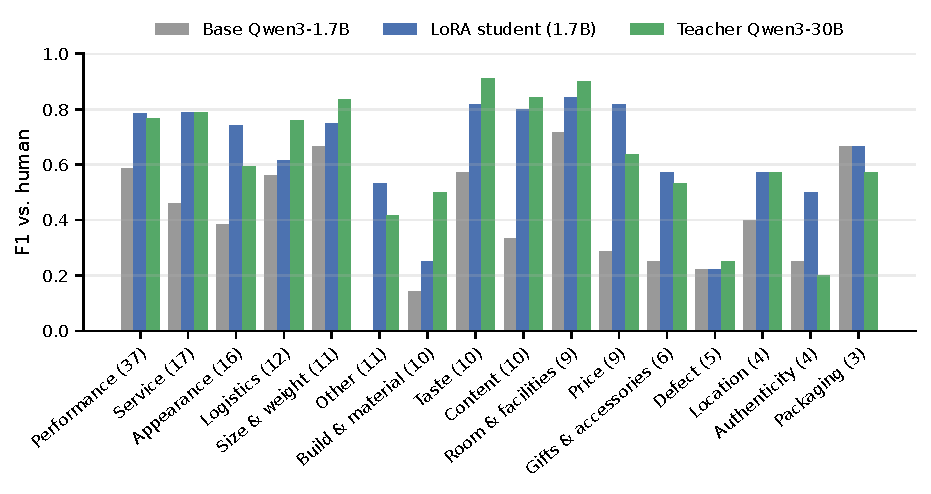
\includegraphics[width=0.85\textwidth]{human_per_aspect_f1}
\caption{Per-aspect F1 against adjudicated human labels on 100 unseen reviews (number of human-labelled occurrences in
brackets). Aspects with few occurrences have unreliable scores.}
\label{fig:human}
\end{figure*}

\begin{figure}[t]
\centering
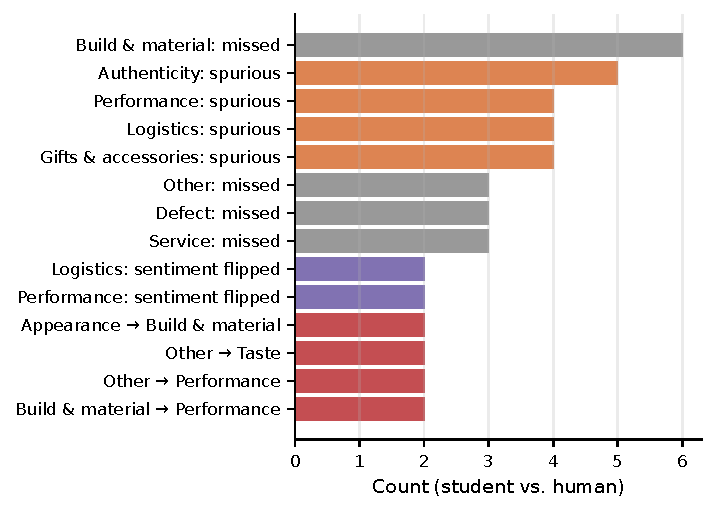
\includegraphics[width=0.92\columnwidth]{human_error_analysis}
\caption{The student's most frequent error types against human labels: missed aspects, spurious aspects, sentiment
flips, and aspect substitutions (human $\rightarrow$ student).}
\label{fig:errors}
\end{figure}

\textbf{Error analysis} (Figs.~\ref{fig:human} and~\ref{fig:errors}). The student's most common errors are missing Build \& material (e.g.\
``the colour runs badly after washing'' labelled only as Performance) and adding a spurious Authenticity aspect when a
customer writes ``this is cheating consumers''. Rare
aspects (Location, Packaging, Authenticity, $n\le4$) have unreliable per-aspect scores.

\subsection{Interactive prototype}
The Gradio~\cite{abid2019gradio} app (Fig.~\ref{fig:demo}) loads the base model \emph{once}; setting $s=0$ in
Eq.~(\ref{eq:lora}) switches every adapter off, so base and fine-tuned outputs are shown side by side without doubling
memory. The page explains \emph{why} an invalid output cannot be used (e.g.\ ``aspect `taste' is not in the allowed
list'') and highlights extracted opinions in the review. On five of its eight built-in examples the base model's output is
invalid while the student's is correct. A dedicated inference thread, a request queue and a warm-up pass make it robust:
12 simultaneous clients all succeeded, at $\approx$4\,s per request.

\begin{figure}[t]
\centering
\IfFileExists{../figures/demo_screenshot.png}{%
  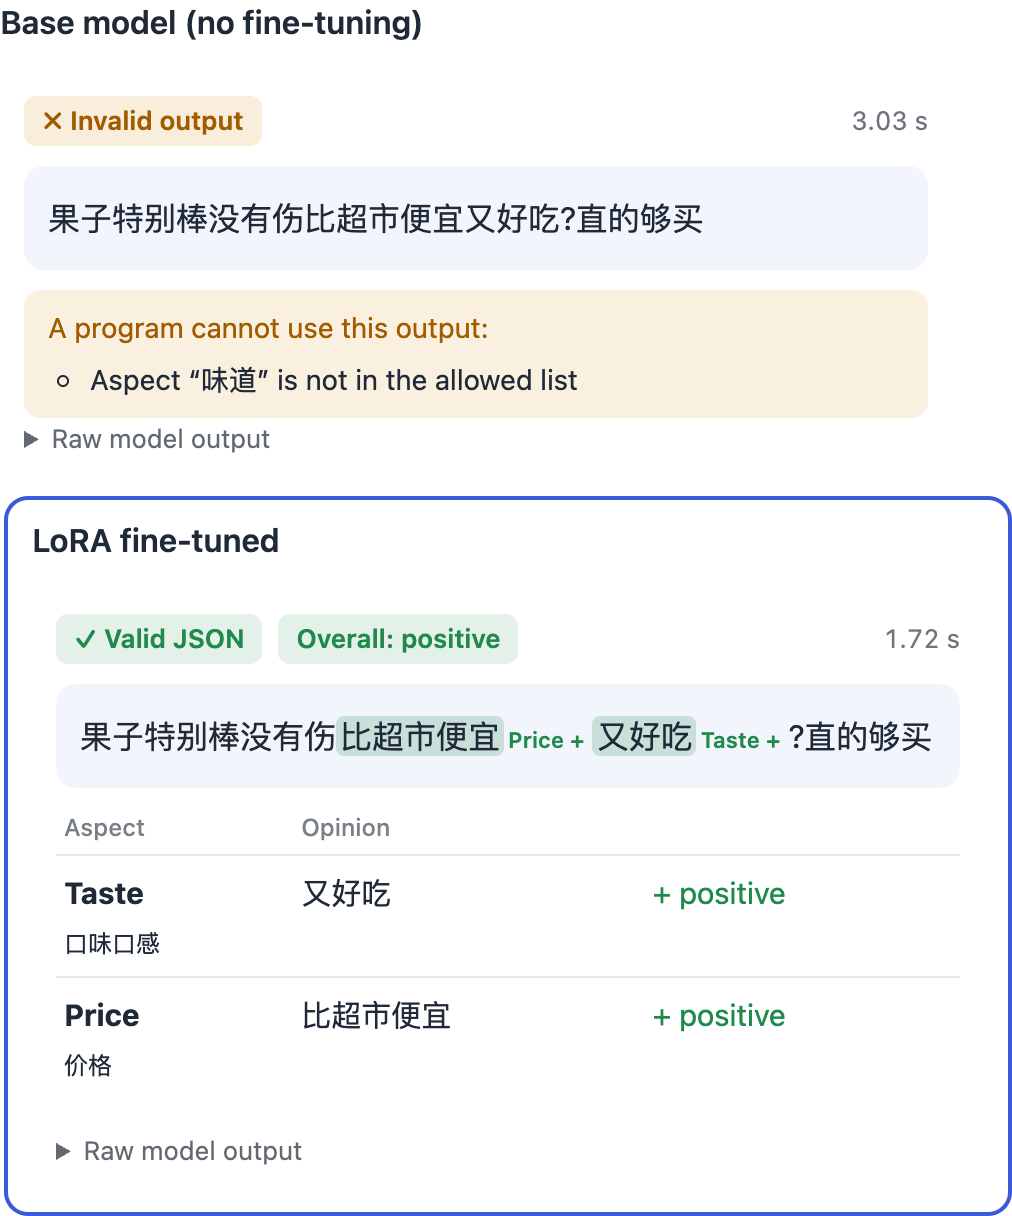
\includegraphics[width=\figwidth]{demo_screenshot}%
}{%
  \IfFileExists{figures/demo_screenshot.png}{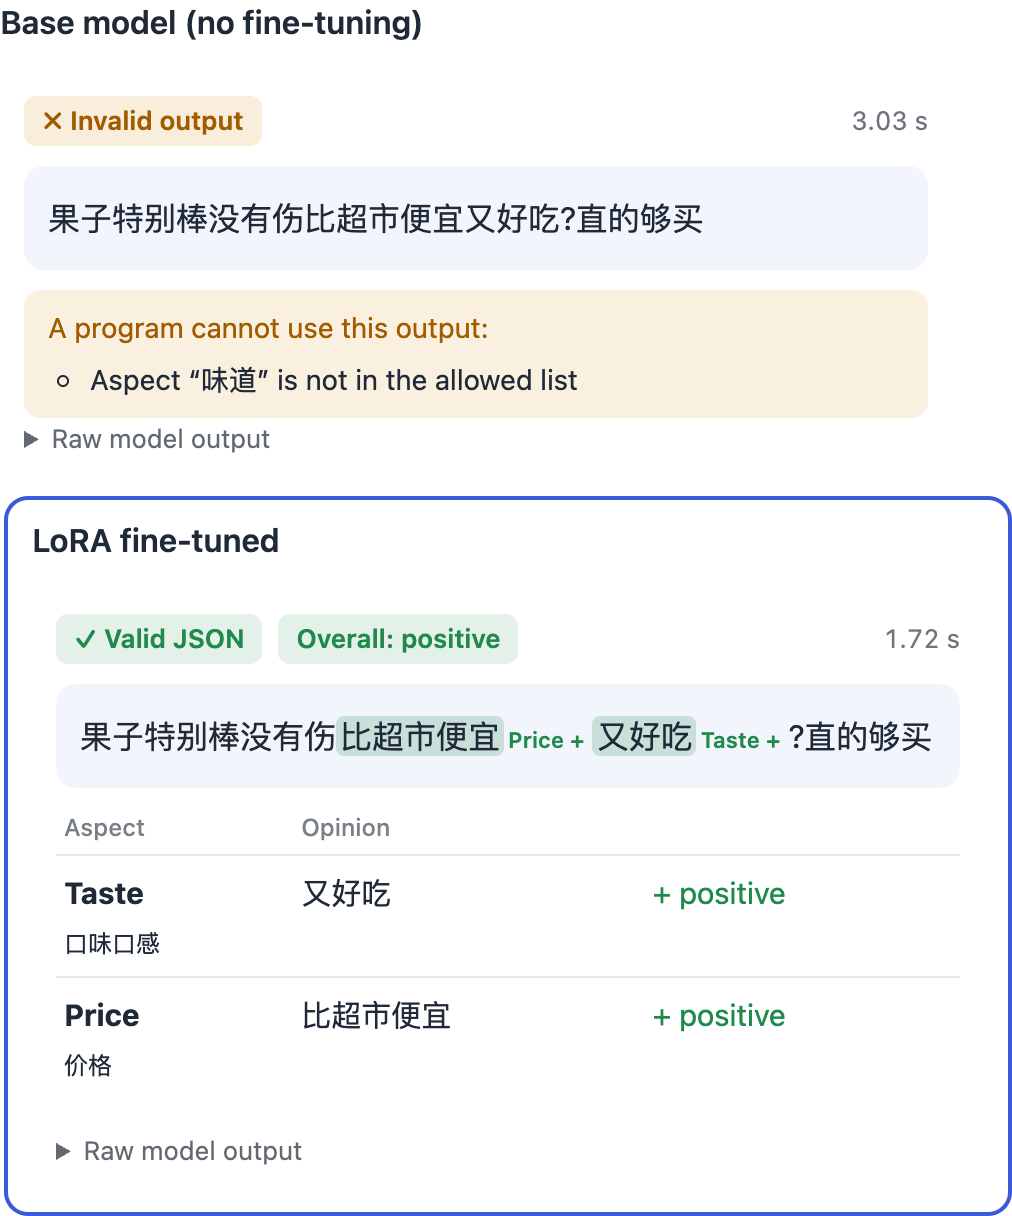
\includegraphics[width=\figwidth]{demo_screenshot}}{%
  \fbox{\parbox[c][3.2cm][c]{0.9\columnwidth}{\centering\small [Gradio screenshot: save as \texttt{figures/demo\_screenshot.png}]}}}%
}
\caption{The Gradio demo: the base model (left) invents an aspect outside the schema; the LoRA model (right) returns
valid, highlighted aspects.}
\label{fig:demo}
\end{figure}

% =====================================================================
\section{Challenges and Conclusion}

\textbf{Overfitting and checkpoint selection.} Our first model trained for three epochs; validation loss bottomed out
after one. We now save a checkpoint every 40 steps and always deploy the one with the lowest validation loss.

\textbf{Ambiguous labels.} The largest single improvement came not from the model but from the label definitions: the
first schema's overlapping ``Quality'' category caused errors that no amount of training could fix. We learned to measure
schema clarity with a second annotator before relabelling the whole dataset, and to pilot new rules on 48--96 reviews
first. Human annotators disagree too (0.644 before adjudication); adjudication is necessary for a trustworthy reference.

\textbf{Memory and speed on a laptop.} Running the 17\,GB teacher together with the demo exhausted GPU memory (Metal
out-of-memory), so heavy jobs are now scheduled one at a time and every long job is resumable. The richer v2 prompt
($\approx$780 tokens) slowed inference from 0.34 to 0.58\,s per review; since the student has internalised the rules, a
much shorter prompt is a promising optimisation. MLX also binds computation to the thread that loaded the model, which
crashed our first multi-threaded web server and motivated the dedicated inference thread.

\textbf{Limitations.} The test reference is teacher-generated. Apart from the final configuration (three seeds) and
the default (two), each configuration was trained once, and even three seeds are few. Of the 100 human-labelled reviews, 80 have a
single annotator and only 20 support the human--model comparison. The sweep varies one factor at a time on a 142-review
validation set, so interactions (e.g.\ lr $5\times10^{-5}$ with $r=4$) are untested.

\textbf{Conclusion.} A 1.7B model fine-tuned with LoRA on 1.8k teacher-labelled reviews, using only a laptop, produces
valid structured output 99--100\% of the time and is statistically indistinguishable from its teacher against human
judgement, with about a fifth of the teacher's weight memory.
Systematic tuning added about 7 F1 points (at least 5.6 for each of three seeds), and the clearest lessons were about data: a precise label schema, a quality filter,
and honest evaluation on data no model has seen.

\textbf{Use of AI tools.} An AI coding assistant (Claude Code) was used to write and debug code and to draft
documentation and parts of this report; all design decisions, annotations and final checks were made by the authors.

\bibliographystyle{IEEEtran}
\bibliography{refs}

\end{document}
